\section{ChimeraX Map Subtraction protocol}
\label{app:chimeraMapSubtraction}%a013

\chimera-based protocol designed to subtract two maps. These two maps can be two density maps experimentally obtained or derived from different computations, including the generation of a density map from an atomic structure. In the context of the \scipion modeling workflow this protocol helps to find out unmodeled densities in a map as a whole or in a specific part of it. In addition, wrong modeled regions can be also identified with this protocol since the atomic structure could doesn't fit to the density map.  
   
 \begin{itemize}
  \item Requirements to run this protocol and visualize results:
            \begin{itemize}
                \item \scipion plugin: \ttt{scipion-em}
                \item \scipion plugin: \ttt{scipion-em-chimera}
            \end{itemize}
  \item \scipion menu:
        \ttt{Model building -> Tools-Calculators} (\ffigure{fig:app_protocol_map_subtract_1} (A))
  
            \begin{figure}[H]
            \centering 
            \captionsetup{width=.9\linewidth} 
            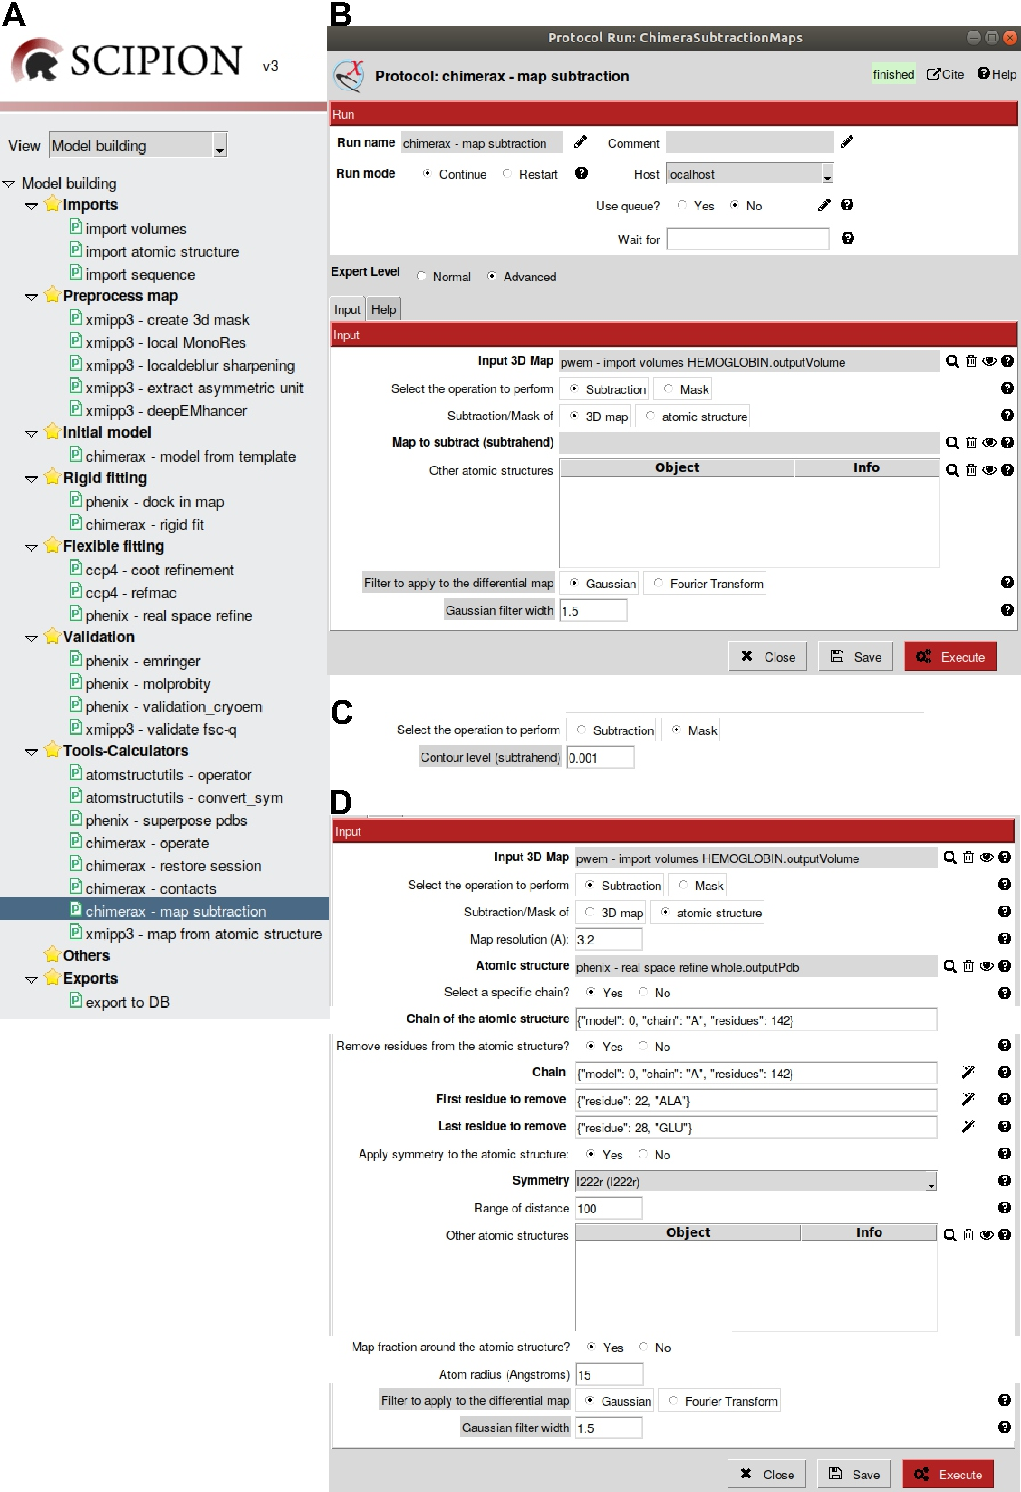
\includegraphics[width=0.85\textwidth]{Images_appendix/Fig309.pdf}
            \caption{Protocol \scommand{chimerax - map subtraction}. A: Protocol location in \scipion menu. B: Protocol form to subtract two maps. C: Param option \ttt{Mask}. D: Protocol form to subtract an atomic structure from a map. All possible params are shown. }
            \label{fig:app_protocol_map_subtract_1}
            \end{figure}
  
  \item Protocol form parameters (\ffigure{fig:app_protocol_map_subtract_1} (B,C,D)):\\ \ttt{Input} section:  

            \begin{itemize}
            \item \ttt{Input 3D Map}: Include here any map previously downloaded or generated in \scipion that you would like to use as minuend of the subtraction operation.
            \item \ttt{Select the operation to perform}: Two possibilities are allowed:
                \begin{itemize}
                        \item \ttt{Subtraction}: Between minuend and subtrahend maps, and you'll obtain the difference. WARNING: Both maps have to be perfectly aligned.
                        \item \ttt{Mask}: The voxel region of the subtrahend greater than a certain level will be masked (\ffigure{fig:app_protocol_map_subtract_1} (C)). The default level is \ttt{0.001} although can be modified with the \ttt{Advanced} param \ttt{Contour level (subtrahend)}. If no level is supplied, \chimera will compute that level value.
                \end{itemize}
            \item \ttt{Subtraction/Mask of}: Select the subtrahend of the subtraction operation. Two possibilities are allowed:
                    \begin{itemize}
                        \item \ttt{3D map}: Any map previously downloaded or generated in \scipion. WARNING: The sampling rate of this map should be identical to the subtrahend's.
                        \item \ttt{atomic structure}: Previously downloaded or generated in \scipion. By selecting this option many new params will interrogate about the structure-derived map that you would like to generate (\ffigure{fig:app_protocol_map_subtract_1} (D)).
                                \begin{itemize}
                                \item \ttt{Map resolution (\AA)}: This is a tricky param and a uniform rule cannot be followed since, although its value is related with the minuend map resolution obtained by computing the \ttt{FSC} in the reconstruction process, local variations of this resolution seem to be involved. As a general rule, start with a resolution value half of the one obtained by the \ttt{FSC} and check your results. Then test other resolution values closer to the one computed by the \ttt{FSC} and compare the results with the previous one. At the end select the resolution that maximizes the difference between the minuend and the subtrahend.
                                \item \ttt{Atomic structure}: Select the atomic structure in the \scipion workflow to generate the called \ttt{molmap\_Map}.
                                \item \ttt{Select a specific chain?}: In case you are interested in generate the sustrahend \ttt{3D map} from the input atomic structure as a whole, answer \ttt{No} to this question. However, answer \ttt{Yes} if you want to derive that map from a specific chain of the atomic structure. If this is the case, a new param (\ttt{Chain of the atomic structure}) will interrogate you about the specific chain that you can select with the help of the wizard on the right.
                                \item \ttt{Remove residues from the atomic structure?}: Select \ttt{Yes} to answer this question in case you'd like to count on a control of density levels to identify the differential density. The aim of this control is identify the density of the removed residues in the differential map. However, be cautious about discarding other densities that could appear in lower resolution areas and have density levels slightly different that the control one. After running the program the \chimera graphics window will open and the atomic structure won't show the removed residues. To make easier the localization of this area, ten residues both upstream and downstream of the removed aminoacids will be highlighted.\\
                                Additional params to interrogate about the residues to be removed are \ttt{Chain}, \ttt{First residue to remove} and \ttt{Last residue to remove}. A wizard on the right helps to select this three elements. WARNING: In case you have already selected a specific chain of the structure to generate the \ttt{3D Map}, this chain will appear by default in the param \ttt{Chain} since the selection of a different chain wouldn't make sense.
                                \item \ttt{Apply symmetry to the atomic structure}: In case your input atomic structure to derive the subtrahend \ttt{3D map} corresponds to the asymmetric unit and you'd like to have the whole atomic structure or at least several adjacent asymmetric units together with the input one, select the option \ttt{Yes}. Otherwise, the subtrahend derived map will only correspond to the asymmetric unit. All \chimera symmetries will be available (\url{https://www.cgl.ucsf.edu/chimerax/docs/user/commands/sym.html}). In case you select symmetries cyclic or dihedral, an additional param will interrogate you about the \ttt{Symmetry Order}. Pay attention to the param \ttt{Range of distance}, set to \ttt{100} by default. This is the distance (in \AA) from the center of the input asymmetric unit to the center of additional allowed asymmetric units, in order to select only the closer ones. You should probably modify the default value to regenerate big maps by applying symmetry.
                                \item \ttt{Map fraction around the atomic structure?}: Select the option \ttt{Yes} if you want to limit the input minuend \ttt{3D Map} to a certain area around the atomic structure. This is the option recommended if you have a big starting map and you'd like to substract a much smaller subtrahend structure-derived map since the visualization of results will be much easier. An additional param, \ttt{Atom radius (\AA)} asks you about the distance around the input structure used to crop the input \ttt{3D Map}. \ttt{15} is the default value. The \chimera-generated map is called \ttt{zone\_Map}.
                                \end{itemize}
                        \item \ttt{Other atomic structures}: Additional atomic structures previously downloaded or obtained in \scipion can be included here to help you identify particular areas of the map or structure. Then, those structures are only informative and won't be used to generate the subtrahend map.
                        \item \ttt{Filter to apply to the differential map}: \ttt{Advanced} parameter to clean the background of the differential map by applying a filter in order to maximize the differences between the minuend and the subtrahend maps, since the differential map usually results quite blurry. This \ttt{filtered\_Map} will always appear together with the \ttt{difference\_Map} when the \chimera graphics window opens. To filter the differential map you can choose between two different filters, \ttt{Gaussian} (with variable width) and based on the \ttt{Fourier Transform}.
                    \end{itemize}
            \end{itemize}
   
  
  \item Protocol execution:
  
  Adding specific volume label is recommended in \ttt{Run name} section, at the form top. To add the label, open the protocol form, press the pencil symbol at the right side of \ttt{Run name} box, complete the label in the new opened window, press OK, and finally, close the protocol. This label will be shown in the output summary content (see below). If you want to run again this protocol, do not forget to set to \ttt{Restart} the \ttt{Run mode}.\\
  Press the \ttt{Execute} red button at the form bottom.\\
  After executing the protocol the \chimera graphics window will open and show the different inputs (maps and atomic structures), as well as the maps generated by the \chimera commands such as \ttt{molmap\_Map}, \ttt{zone\_Map}, \ttt{difference\_Map} and \ttt{filtered\_Map}. Most of the outputs are already saved in \scipion, however you can perform any operation of your preference and save the new results before closing \chimera. Common commands of \chimera-\scipion communication are allowed in this case: \ttt{scipionwrite}, \ttt{scipionss} and \ttt{scipioncombine}.
  
  \item Visualization of protocol results:
  
  After exiting the protocol, press \ttt{Analyze Results} and the $ChimeraX$ graphics window will open with every saved elements, inputs and outputs, which might be distinct acording to the inputs. In addition to items mentioned in the previous paragraph, the atomic structure without the removed residues used as a control, called \ttt{mutated\_Atom\_structure} will be also shown overlapping the input structure.\\
  
  By pressing the left black arrow shown in the \ttt{Summary Output} the saved maps can be also opened with $ShowJ$, the default \scipion viewer that shows each map's \ttt{slices} (\url{https://github.com/I2PC/scipion/wiki/ShowJ}).
   
   \item Summary content:
    
    \begin{itemize}
     \item Protocol output (below \scipion framework):\\
     For each map: \ttt{chimerax - map subtraction -> ouput map name};\\ \ttt{Volume (x, y, and z dimensions, sampling rate)}.\\
     For each atomic structure: \ttt{chimerax - map subtraction -> output atomic structure name};\\ \ttt{AtomStruct (pseudoatoms=False, volume=False}).\\
     \item \ttt{SUMMARY} box:\\\ttt{Produced files}:\\List of output map names\\ \ttt{we have some result} 
    \end{itemize}
  
  \end{itemize}


\subsubsection*{USE CASES}
\begin{itemize}
                \item \ttt{Use Case 1: Detection of remnant density in the penton region of the human adenovirus HAdV-F41 density map (\ttt{EMDB ID EMD-10768}, \citep{PerezIllana2020})}\\
                Aim: Run the \scipion workflow depicted in \ffigure{fig:app_usecase_mapsubtract_1} (A). The output of protocols 1, 2 and 3 can be seen in the \chimera viewer by pressing \ttt{Analyze Results}.
                \begin{itemize}
                        \item In the \ffigure{fig:app_usecase_mapsubtract_1} (B) appears the whole adenovirus map, output of protocol 1. To visualize this map write in the \chimera command line:\\
                        \\
                        \ttt{volume \#2 region all showOutline false}\\
                        \\
                        and adjust level densities according with indicated in the shown \ttt{Volume Viewer}.
                        \item In the \ffigure{fig:app_usecase_mapsubtract_1} (C) the extracted asymmetric unit is shown, overlapped to the whole map, as output of protocol 2. To visualize these maps, in addition to the previous \chimera command line and the adjustment of map levels indicated below, modify the transparency of the whole map writing:\\
                        \\
                        \ttt{volume \#2 transparency 0.8}
                        \item Finally, the \ffigure{fig:app_usecase_mapsubtract_1} (D) details the atomic structure of the biological asymmetric unit obtained by modeling as output of protocol 3 (\ttt{PDB ID 6YBA}). Select \ttt{Atoms -> Hide} and \ttt{Cartoons -> Show} to change to ribbons the view of the structure. The overlapping of this structure to the geometrical map asymmetric unit allows to observe the area (5, dotted blue circle) where the penton is located and we will try to see a remnant density. To visualize the map, write in the command line:\\
                        \\
                        \ttt{volume \#2 transparency 0.9}
                \end{itemize}

                            \begin{figure}[H]
                            \centering 
                            \captionsetup{width=.9\linewidth} 
                            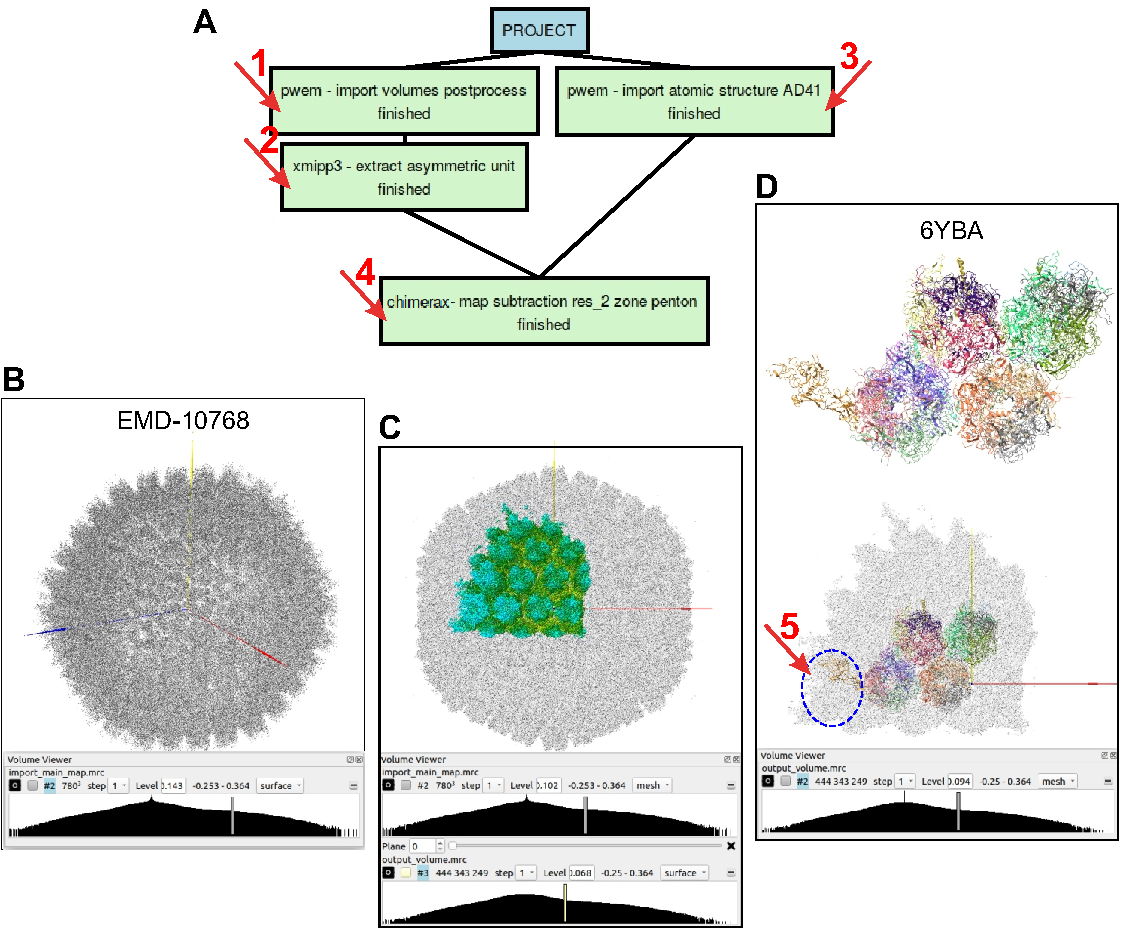
\includegraphics[width=.9\textwidth]{Images_appendix/Fig310.pdf}
                            \caption{(A) \scipion workflow showing protocols 1, 2, 3 and 4. (B) Adenovirus HAdV-F41 map image. (C) Map geometrical asymmetric unit extracted from the adenovirus map. (D) Adenovirus atomic structure of the biological asymmetric unit overlapped to the geometrical map unit. }  
                            \label{fig:app_usecase_mapsubtract_1}
                            \end{figure}
                To look for remnant densities in the penton area we have to complete the \scommand{chimerax - subtraction} protocol with the indicated params (\ffigure{fig:app_usecase_mapsubtract_2}. Remark that in this case we have selected half of input \ttt{3D Map} resolution (4 \AA) although other values could be tested. The only chain of the penton in the atomic structure of the asymmetric structure is the chain \ttt{M}, inside the dotted blue circle of \ffigure{fig:app_usecase_mapsubtract_1} (D), and 8 residues will be removed as a control of density levels. In addition, icosahedral \ttt{I222r} symmetry will be applied to the selected chain in order to complete the five units of the penton. In order to visualize better the map difference, a map fraction around the atomic structure is selected.
                            
                            \begin{figure}[H]
                            \centering 
                            \captionsetup{width=.9\linewidth} 
                            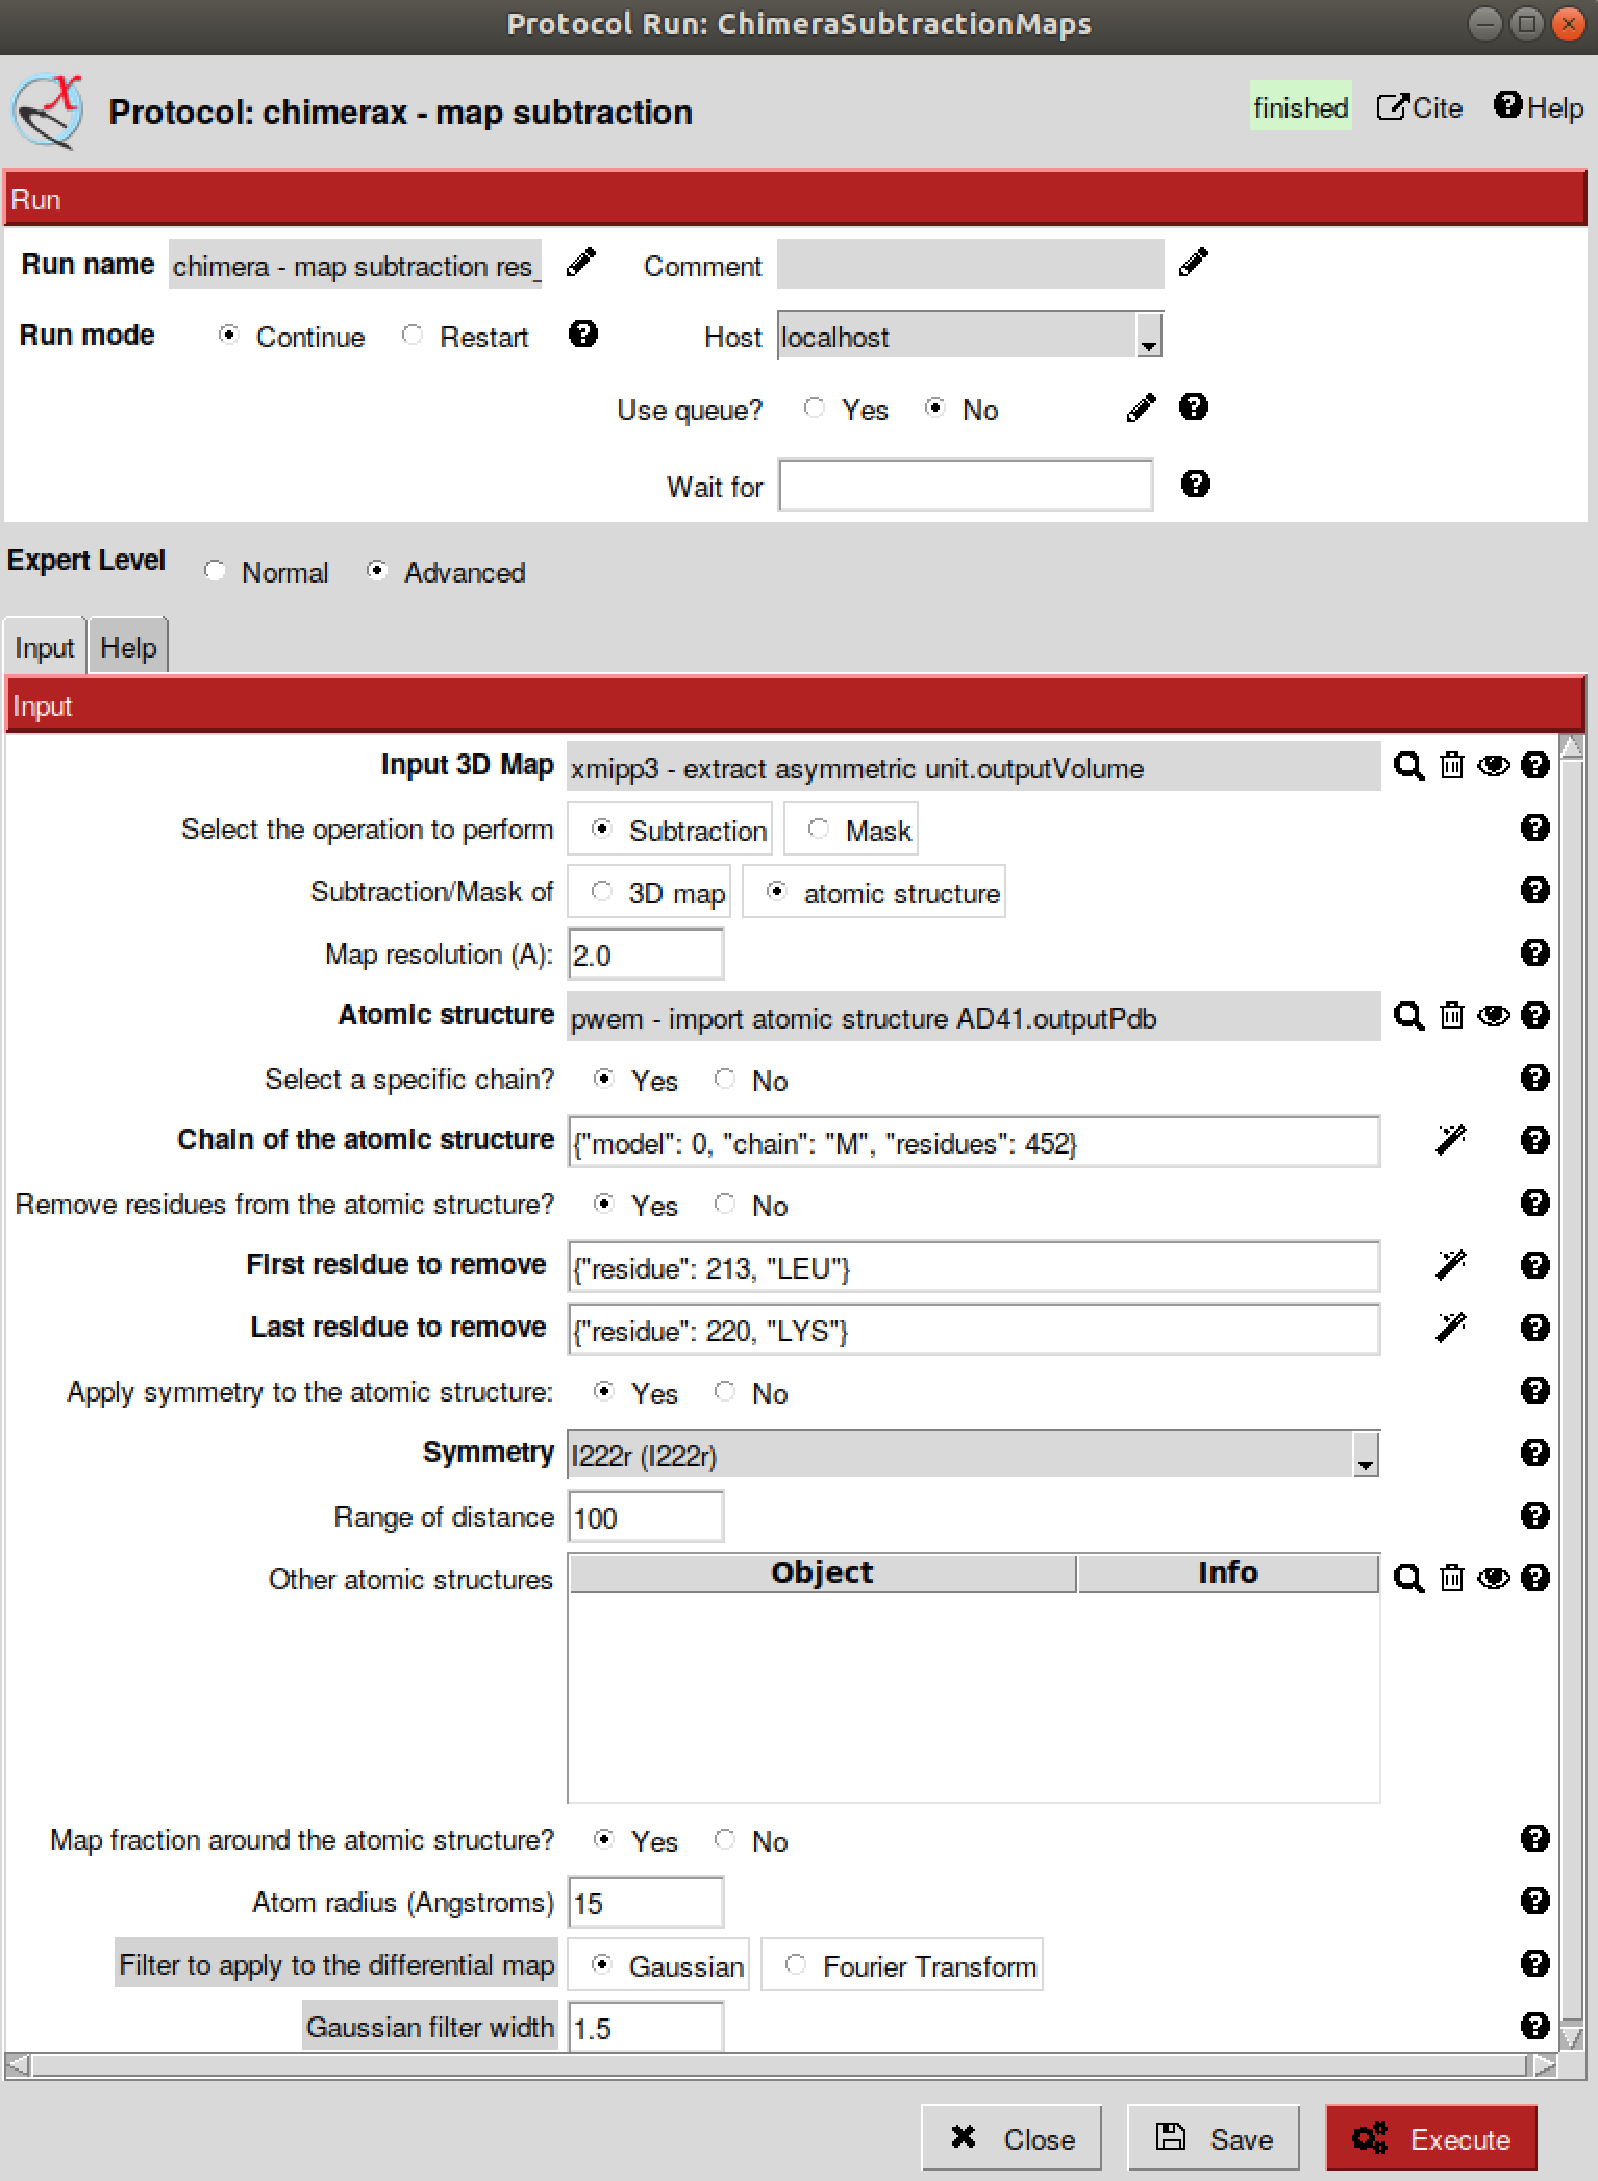
\includegraphics[width=.50\textwidth]{Images_appendix/Fig311.pdf}
                            \caption{Completing the protocol \scommand{chimerax - subtraction} to find renmant densities in the penton area of the adenovirus map.}  
                            \label{fig:app_usecase_mapsubtract_2}
                            \end{figure}
                Protocol execution: Follow the general procedure shown above (Protocol execution section) and the \chimera graphics window will open. At this point several maps and atomic structures will be shown, as the \ttt{Models} panel indicates (\ffigure{fig:app_usecase_mapsubtract_3} (C, top)). Have a look to each map and structure to identify them and play with the density levels to maximize the differences between the input \ttt{3D Map} restricted to the penton area (\ttt{zone\_Map}) and the penton atomic structure-derived map (\ttt{molmap\_chainM\_Map}). The \ffigure{fig:app_usecase_mapsubtract_3} images A and B show the difference \ttt{filtered\_Map} in the penton side (A) and upper (B) views, respectively, according to the density level observed on the \ttt{Volume Viewer} panel (C, middle). Red arrows point at the densities associated to the removed residues used as a density control. The adjacent ten residues to the removed ones upstream and downstream are green-highlighted. The penton upper view (B) was obtained opening the \chimera main menu (\ttt{Tools -> General -> Side View} and setting the view as indicated (C, botton). From these results we can conclude that a remnant density in the upper part of the penton, if exits, it is not so evident.
                            \begin{figure}[H]
                            \centering 
                            \captionsetup{width=.9\linewidth} 
                            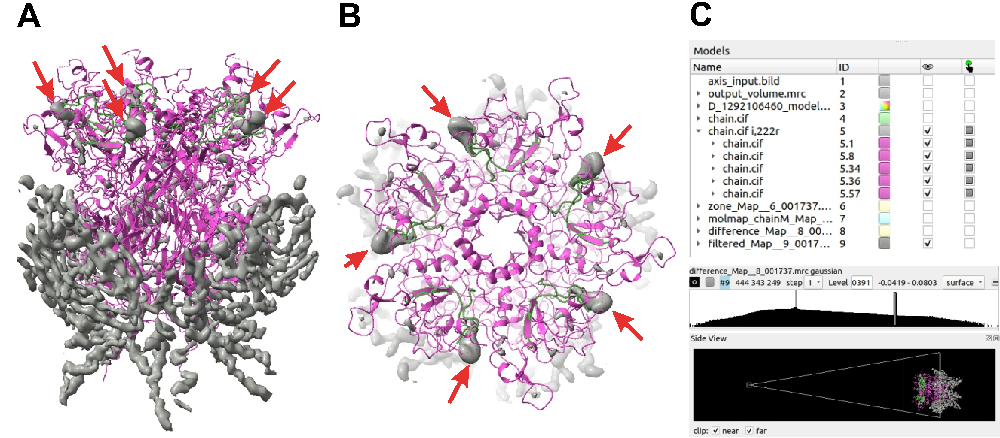
\includegraphics[width=.9\textwidth]{Images_appendix/Fig312.pdf}
                            \caption{(A) Side view of the adenovirus penton atomic structure (magenta) and the gaussian filtered difference map (grey). (B) Upper view. (C) From top to bottom, \chimera \ttt{Models} panel, \ttt{Volume Viewer} panel, specified for the gaussian filtered difference map, and \ttt{Side View} panel, respectively.}  
                            \label{fig:app_usecase_mapsubtract_3}
                            \end{figure}
                With the exception of the input adenovirus biological asymmetric unit atomic structure, the rest of elements shown in the \chimera graphics window will also appear in the \chimera viewer that opens pressing \ttt{Analyze results}. Consider then the possibility of performing additional operations and saving them with the \ttt{scipionwrite} command before closing the graphics window. After exiting the protocol you can visualize your results.
                
                \item \ttt{Use Case 2: Since the asymmetric unit of the human adenovirus HAdV-C5 atomic structure contains a small chain called \ttt{X} (\ttt{PDB ID 6B1T}), we'd like to check if there is a remnant density in the previous human adenovirus HAdV-F41 density map (\ttt{EMDB ID EMD-10768}) that could be interpreted as the HAdV-C5's chain \ttt{X}.}\\
                Aim: Run the \scipion workflow depicted in \ffigure{fig:app_usecase_mapsubtract_4} (A) to inspect for remnant densities around the area covered by the hexons in the biological asymmetric unit area of the adenovirus map (A, 6). The output of all protocols can be seen in the \chimera viewer by pressing \ttt{Analyze Results}. 
                \begin{itemize}
                        \item In the \ffigure{fig:app_usecase_mapsubtract_1} (B, C, D) you also have the output of protocols 1, 2 and 3. 
                        \item The output of the protocol 4 shows the atomic structure of human adenovirus HAdV-C5. Select \ttt{Atoms -> Hide} and \ttt{Cartoons -> Show} to change to ribbons the view of the structure. This structure was fitted to the map asymmetric unit of adenovirus HAdV-F41 by using the protocol \scommand{chimerax - operator} (6) and the result of this oputput, overlapped to the geometrical map asymmetric unit, is shown in \ffigure{fig:app_usecase_mapsubtract_4}(B). To visualize this map write in the \chimera command line:\\
                        \\
                        \ttt{volume \#2 transparency 0.8}\\
                        \\
                        and adjust level densities according with indicated in the shown \ttt{Volume Viewer} (\ffigure{fig:app_usecase_mapsubtract_4} (D)). Select \ttt{Atoms -> Hide} and \ttt{Cartoons -> Show} to change to ribbons the view of the structure.
                        \item The output of protocol 5 details some small chains of \ttt{ALA} residues previously traced in the remnant density of the adenovirus HAdV-F41. They are used as a control to be sure that we identify new densities previously unmodeled. Since they are very small we have depicted them selecting \ttt{Styles -> Stick} and overlapped to the geometrical map asymmetric unit (\ffigure{fig:app_usecase_mapsubtract_4} (C) with the same transparency and map adjustment shown in (B).
                        \end{itemize}
                            \begin{figure}[H]
                            \centering 
                            \captionsetup{width=.9\linewidth} 
                            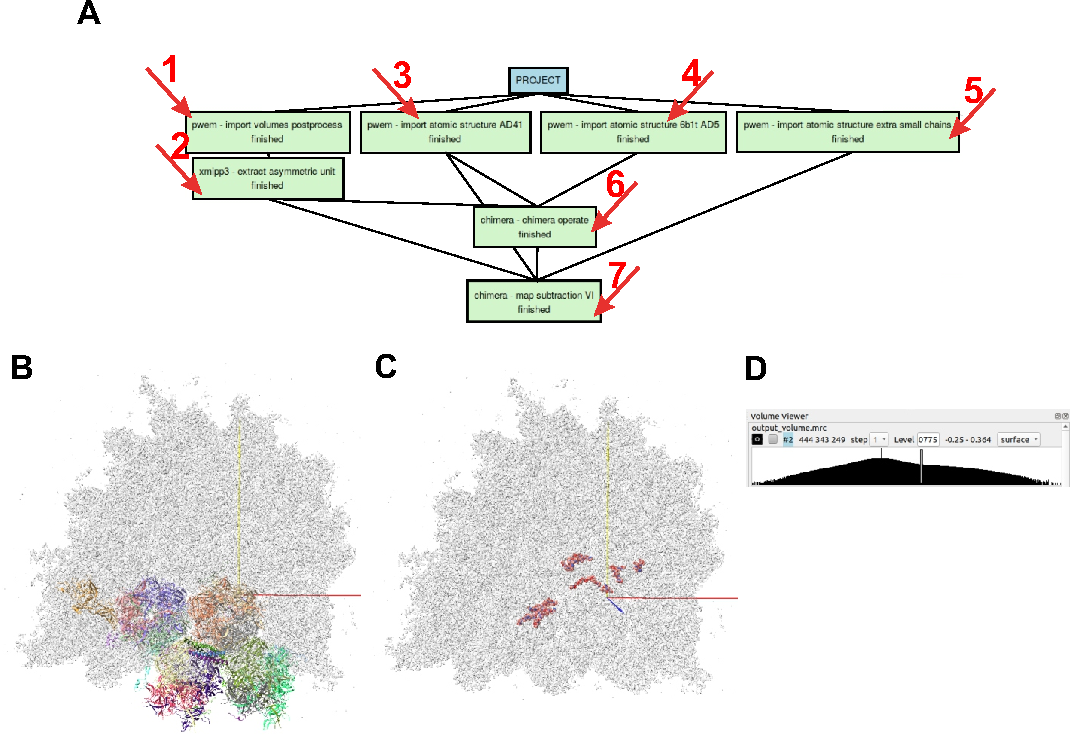
\includegraphics[width=.9\textwidth]{Images_appendix/Fig314.pdf}
                            \caption{(A) \scipion workflow showing protocols 1-7. (B) HAdV-F41 adenovirus geometrical map asymmetric unit (grey) and, fitted to it, the atomic structure of the biological asymmetric unit atomic structure of HAdV-C5 adenovirus (colored). (C) HAdV-F41 adenovirus geometrical map asymmetric unit (grey) and some small aminoacid chains previously traced in the remnant density, imported in the protocol 5 (colored). (D) Level of density selected to visualize the map in B and C. }  
                            \label{fig:app_usecase_mapsubtract_4}
                            \end{figure}
                         To look for remnant densities in the area of hexons we have to complete the \scommand{chimerax - subtraction} protocol with the indicated params (\ffigure{fig:app_usecase_mapsubtract_5}. As in the previous use case, we have selected half of input \ttt{3D Map} resolution (4 \AA) although other values could be tested.\\Taking into account that the remnant densitities could be quite inconspicuous we are going to use two different controls this time. One of them will be, as in the previous use case, the deletion of 5 residues of hexon chain \ttt{D}, in a region presumed to be quite close to the remnant density that we are looking for. The second control will be some small aminoacid chains previously traced in the remnant density since we'd like to discriminate between this density and other new one and unmodeled. These extra small changes have to be included in the form param \ttt{Other atomic structures}.\\ Although this time we do not have to consider a specific chain or applying symmetry, since we have to look for a chain similar to HAdV-C5 adenovirus chain \ttt{X}, to include in the form param \ttt{Other atomic structures} the structure 6B1T fitted to the geometrical map asymmetric unit, as shown in \ffigure{fig:app_usecase_mapsubtract_4} (B), and obtained from protocol 6 (A), is quite recommendable. 
                            
                            \begin{figure}[H]
                            \centering 
                            \captionsetup{width=.9\linewidth} 
                            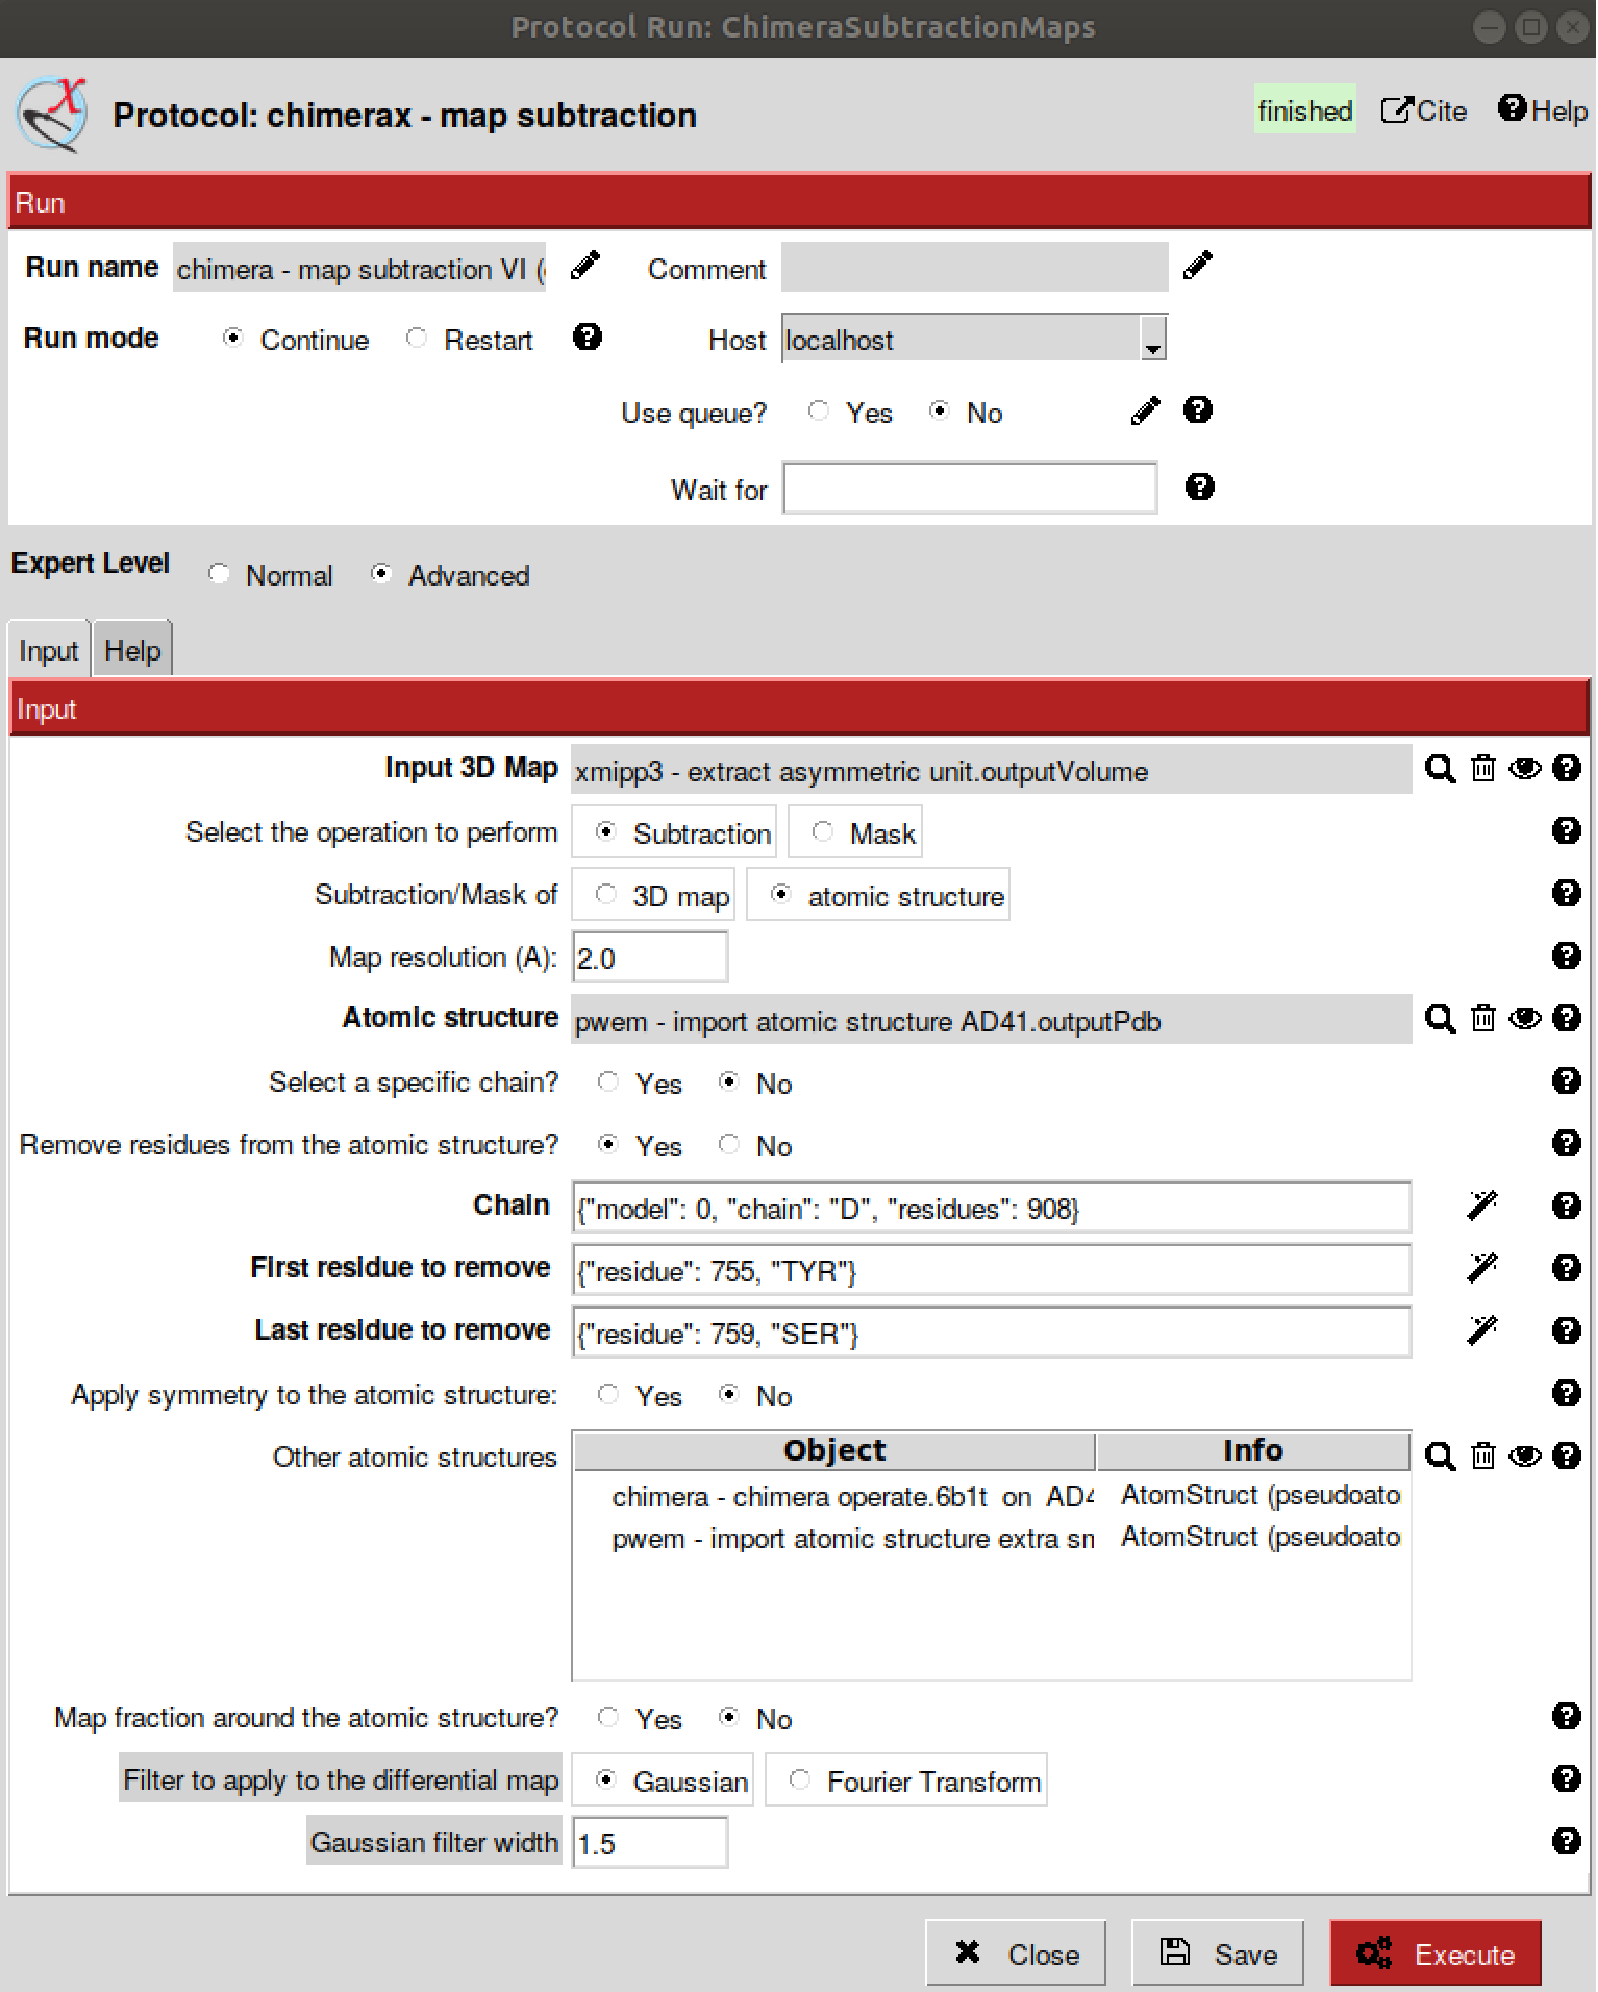
\includegraphics[width=.50\textwidth]{Images_appendix/Fig313.pdf}
                            \caption{Completing the protocol \scommand{chimerax - subtraction} to find renmant densities in the biological asymmetric unit area of the adenovirus map.}  
                            \label{fig:app_usecase_mapsubtract_5}
                            \end{figure}
                            
                        Protocol execution: Follow the general procedure shown above (Protocol execution section) and the \chimera graphics window will open. At this point several maps and atomic structures will be shown, as the \ttt{Models} panel indicates (\ffigure{fig:app_usecase_mapsubtract_6} (A, bottom)), except the \iii{model} \ttt{\#6}. Have a look to each map and structure to identify them and play with the density levels to maximize the differences between the input \ttt{3D Map} (\ttt{output\_volume.mrc}) and the \ttt{6YBA} atomic structure-derived map (\ttt{molmap\_Map}). The \ffigure{fig:app_usecase_mapsubtract_6} (A) show the difference \ttt{filtered\_Map} obtained. The zoom in on the framed area displays in detail the difference considering two different map levels (B and C). To have this view, besides select the molecules to show according to the \ttt{Models} panel (A, bottom), write in \chimera command line:\\
                        \\
                        \ttt{volume \#2 transparency 0.8}\\
                        \\
                        \ttt{select \#4/X}\\
                        \\
                        \ttt{save /tmp/6b1t\_chainX.cif format mmcif models \#4 selectedOnly true}\\
                        \\
                        \ttt{open  /tmp/6b1t\_chainX.cif }\\
                        \\
                        \ttt
                        HAdV-C5 adenovirus chain \ttt{X} can be visualized as \iii{model} \ttt{\#6}.  
                        
                        
                        The results, described in \ffigure{fig:app_usecase_mapsubtract_6}, doesn't demonstrate a clear continuous density in the proximity of the HAdV-C5 adenovirus chain \ttt{X}. Although not very evident, it could be there. Then we cannot conclude that it doesn't exit, only that we were unable to identify it.
                            
                            \begin{figure}[H]
                            \centering 
                            \captionsetup{width=.9\linewidth} 
                            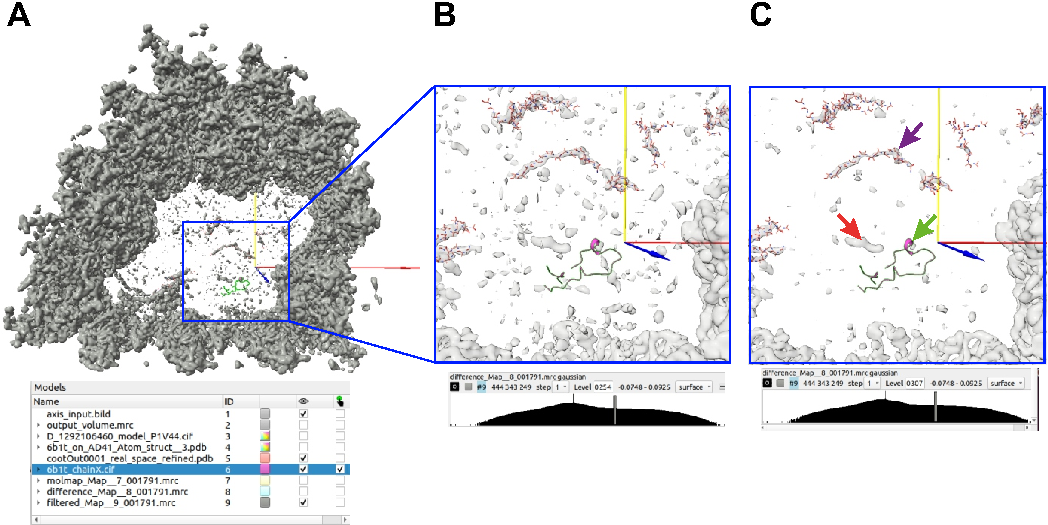
\includegraphics[width=.9\textwidth]{Images_appendix/Fig315.pdf}
                            \caption{(A) Gaussian filtered difference map (grey) of adenovirus HAdV-F41 asymmetric unit (top) and \ttt{Models} panel of items loaded in \chimera including the \iii{model} \ttt{\#6} (bottom). (B) Zoom in on the subtracted area with the map density level indicated in the \ttt{Volume Viewer} below . (C) Idem with a higher cleaning of the background. The red arrow points at the control density. The green arrow points at the HAdV-C5 adenovirus chain \ttt{X}. The purple arrow points at one of the adenovirus HAdV-F41 small chains previously traced.}  
                            \label{fig:app_usecase_mapsubtract_6}
                            \end{figure}
                
\end{itemize}
